% $Rev: 356 $:			Revision of last commit
% $Author: mg483 $:		Author of last commit
% $Date: 2018-05-24 16:05:25 +0100 (Thu, 24 May 2018) $:    Date of last commit

\documentclass[twoside,12pt,titlepage,a4paper]{article}
\usepackage{url}
% kentHarvard requires natbib
\usepackage{natbib}
% add line numbers
\usepackage{lineno}
\usepackage[final]{pdfpages}
\usepackage{xcolor}
\linenumbers
\definecolor{periwinkle}{rgb}{0.8, 0.8, 1.0}
\renewcommand{\linenumberfont}{\normalfont\bfseries\small\color{periwinkle}}
\usepackage[pass]{geometry}
\usepackage{graphicx}
\renewcommand{\baselinestretch}{1.3}
\usepackage{todonotes}
% An empirical comparison of the structure of configuration files of continuous integration and build systems
\title{Usage and structure of continuous integration as configuration?}
\author{Joseph Ling\\\vspace{10mm}
       \url{jl653@kent.ac.uk} \\ \vspace{5mm}
       
\includegraphics[scale=0.6]{Kent_Comp_294_RGB} \\
       School of Computing \\
       University of Kent \\
       United Kingdom \\ \vspace{10mm} \\ Word Count: 6,100}
\begin{document}

\newgeometry{hmarginratio=1:1}    %% make layout symmetric
\maketitle
\restoregeometry              %% restore the layout

\begin{abstract}
This paper describes a simple heuristic approach to solving large-scale
constraint satisfaction and scheduling problems.  In this approach one
starts with an inconsistent assignment for a set of variables and
searches through the space of possible repairs. The search can be guided
by a value-ordering heuristic, the {\em min-conflicts heuristic}, that
attempts to minimize the number of constraint violations after each
step.  The heuristic can be used with a variety of different search
strategies.  We demonstrate empirically that on the $n$-queens problem, 
a technique
based on this approach performs orders of magnitude better than
traditional backtracking techniques.  We also describe a
scheduling application where the approach has been used successfully.  A
theoretical analysis is presented both to explain why this method works
well on certain types of problems and to predict when it is likely to
be most effective.
\end{abstract}

\section{Introduction}
\label{Introduction}

https://arxiv.org/ftp/arxiv/papers/1703/1703.07019.pdf

Continous integeration (CI) is becoming more popular over the last few years. This can be seen by how major version control hosting services Github, Bitbucket and Gitlab have all started to or have been improving their CI product. In terms of research, configuration as code \cite{Rahman2019} and continuous integeration \cite{Copeland2010} with \cite{Shahin2017} demonstrating breadth of the research.

Continous integeration is a process of automatically running compiling, running tests and checking that the product works. This is can be combined with Continous Delivery where the product is deployed or released after it has gone through CI. 

This can get complicated quickly therefore configuration as code (or infrastructure as code) is used to configure it. The main kind of configuration format used for this is yaml (reference to what it is??) followed by xml and java based scripting formats.


In terms of looking at usage we are going do a similar look at the data as did \cite{Hilton2016}. The importanat aspect will be looking at how usage has changed over the last 5 years along with looking more closely at which repositories are more likely to use CI/CD. For this we are going to focus on the following research questions:
\begin{itemize}
  \item usage of CI vs non usage
  \item multiple CI used
  \item per language CI usage
  \item stars, subscribers and commits for likehood of using CI
\end{itemize}

This should give us a better understanding of the sample of repositories from Github. From there we look at the structure of the configuration files to understand how certain aspects of it are used.
\begin{itemize}
  \item configuratizon errors when loading the config (just yaml parsing errors atm)
  \item how are comments used in the configuration?
  \item  how scripts with the configuration files? (need to elloborate more on this one)
\end{itemize}

A key aspect is that these questions do not look too deeply into the individual implementation of each CI system. This is because there are already some good papers looking \cite{Gallaba2018} at this but in order to be able to compare the different configuration types it is important to compare similar attributes (there is also a time factor in here as well). 

\section{Previous Works}
\label{config as code}

Configuration as code or infrastructure as code has been an increasing area of research over the last few years. There seems to be slightly more research in infrastructure as code \cite{Rahman2019}. The has been a focus on Puppet and Chef, for example in \cite{Sharma2016} looks at code quality by the measure of "code smell" of Puppet code. This tackles the problem by defining by best practices and analyzing the code against that. In the case of \cite{Cito2017} it uses the docker linter in order to be able to analyse the files. 
For the continous integeration systems we pick we will look into the tooling around that to aid the analysis.

\label{Continous integeration}

\cite{Hilton2016}

\section{Methodology}
\label{methodology}

In order to get repositories with CI/CD configuration from Github we have a number of approaches. The first is too use the search for particular files but this is limited to only 1000 results. The alternative is to search for repositories and we bypass the 1000 result limit to an extent by getting results for every 'star' count (stars are used to like or upvote a repository). Although this will be giving us a lot of results it will still only be a sample of the population but will give us a wider range of results. As their is rate limiting multiple github api keys can be used to speed up the scraping of data (ghtorrent could also be used to speed up the process I think).

After we have got a repository we need to get the CI/CD files from it. This is fairly easy as the CI/CD systems normally require a strict naming convention and location within the repository. However as most of them are yaml based you can have ".yml" and ".yaml" and users can use all sorts of mixtures of upper and lower case. We try to account for this but won't get every scenario. This combined with the fact that we are only looking for top configuration files based on \cite{Github2017} along with github actions and azure pipelines. Is why we also check repositories for their ReadMe.md file to check if it has a build tag.

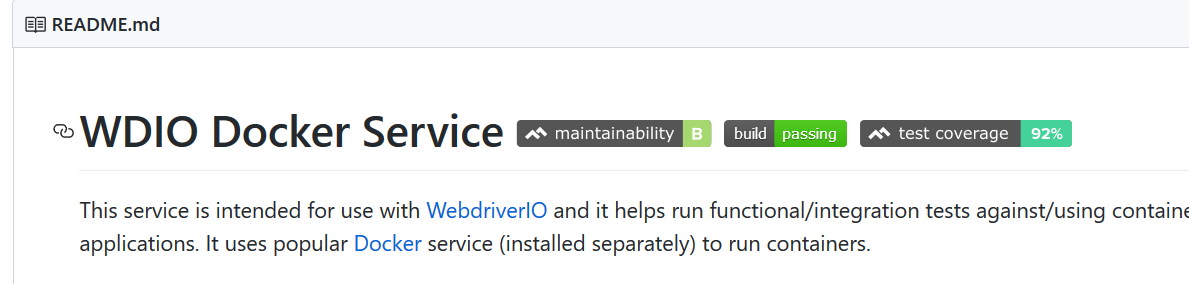
\includegraphics[scale=0.5]{2020-01-30-08-29-04.png}
\todo[size=\scriptsize]{where did this image come from?? reference it man}

In doing so it should give a wider net when sampling and help to understand when a CI system is either not using configuration as code or using a different CI system.

There are dangers in scraping data off github in terms of assumptions to do with the population as found in \cite{Kalliamvakou2014}. In Github you can fork a repository which copies in order to remove these we check for fork flag on the repository. This causes are dataset to go from NUMBER to OTHER\_NUMBER.

Additionally the assumption that all repositories are of programming projects with code in them is wrong. A number of repositories can be used for storage, experimental, academic and other things. However they to all some extent can use CI/CD for their work as a number of books were found when looking through the dataset could use CI/CD. \todo[size=\scriptsize]{Analyse of readme can be used to try and classify but I don't think that is necessary. I think the key factor is that any concluding remarks anywhere take this into account.}

\todo[size=\scriptsize]{Additionally the paper suggests looking a for recent commits but I don't think that is necessary just yet... but would be a good indication later on size/dating the projects when comparing CI/CD systems.}

Tooling for the configuration files, I looked into Travis, Github Actions and Jenkins to work out whether or not it could aid in the research or not. As a key part of understanding the first relies on knowing whether or not it is valid. 
In terms for travis there is currently two parsers to validate the configuration. One which is depracted since 2017 (https://github.com/travis-ci/travis-yaml/) the other which is currently in development (https://github.com/travis-ci/travis-yml). Both didn't provided the necessary results with the most recent one not being able to handle default fields.
For Github Actions as it's still a new tooling for it hasn't been developed outside of the Github editor web page (https://github.community/t5/GitHub-Actions/YAML-validator-for-Github-Actions-possible-expansion-of/td-p/29557).
For Jenkins which is older solution allows validation through http/ssh request to the Jenkins server (Gitlab follows this style as well) \cite{JenkkinsDocs2020} \cite{GitlabDocs2020}. This could work well although would require setting up a server for each configuration type and might not validate if varaibles from the config aren't defined on the server. As well as it would be best to be able to validate them all or none of them in terms of being able to compare results easily.

\section{Usage of CI}

\vspace*{-0.05in}
\subsection{configuration errors when loading the config (just yaml parsing errors atm)}
\vspace*{-0.05in}

This leads us to get the following data:


    \begin{table}[h]
\begin{tabular}{|l|l|l|l|l|}
\hline
    CI/CD & \textbf{count} & \textbf{repos with config} & \textbf{no. multiple} & \textbf{multiple percent}   \\ \hline
config file(s) &           12128     & 38.51\%                                & 1675          & 13.81\%             \\ \hline
found in ReadMe & 873     & 2.77\%                                &             &             \\ \hline
none found &            18493     & 58.72\%                                &             &             \\ \hline
\end{tabular}
\caption[Percentage of CI used for projects]{Percentage of CI used for projects}
\end{table}
    



A repository on github is like a folder so can contain any number of configuration files in it. Therefore we can get any number of configuration files in that folder. This is taken into account with the second pair of columns for the first row. It demonstrates that their a large number of repositories with multiple kinds of configuration (todo make sure that github actions multiple file thing isn't calculated here).

The next row is for when we couldn't pick up the configuration used for CI/CD and check the ReadMe.md file for build status tag. 

The final row is shows the repositories that either don't have any configuration or no configuration that could be found.

However that doesn't give us too much insight into the dataset. Here is a graph showing the subscribers plotted against the number of stars. The key here to understand is not potentially any correlation but to see the spread of data that the table is showing. 
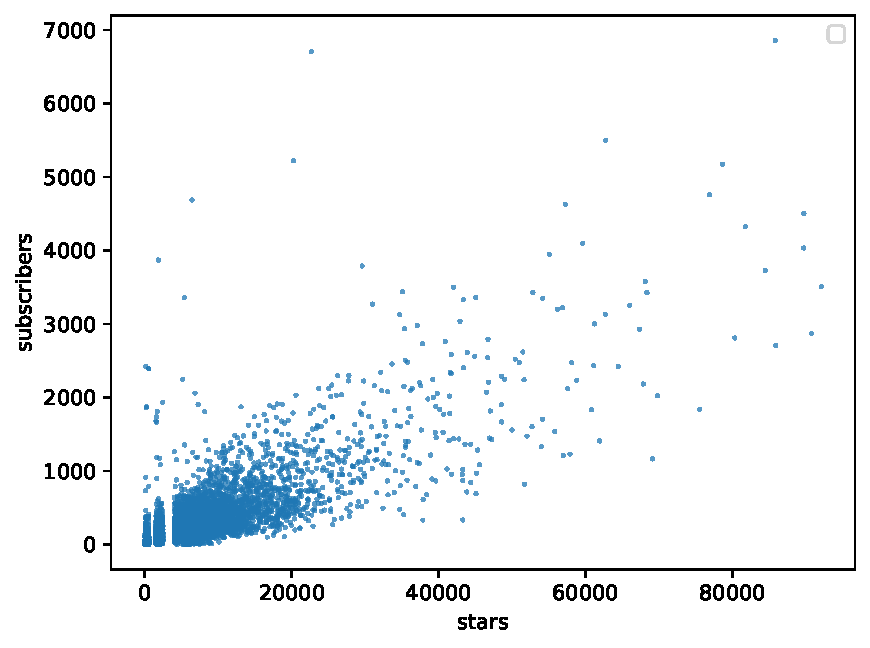
\includepdf[pages=-,pagecommand={},width=\textwidth]{../src/sub vs stars.pdf}

The second graph helps give a understanding to the give a depth of the data for where the graph is just blue. This is because on Github you get more repositories with smaller star counts than large ones.

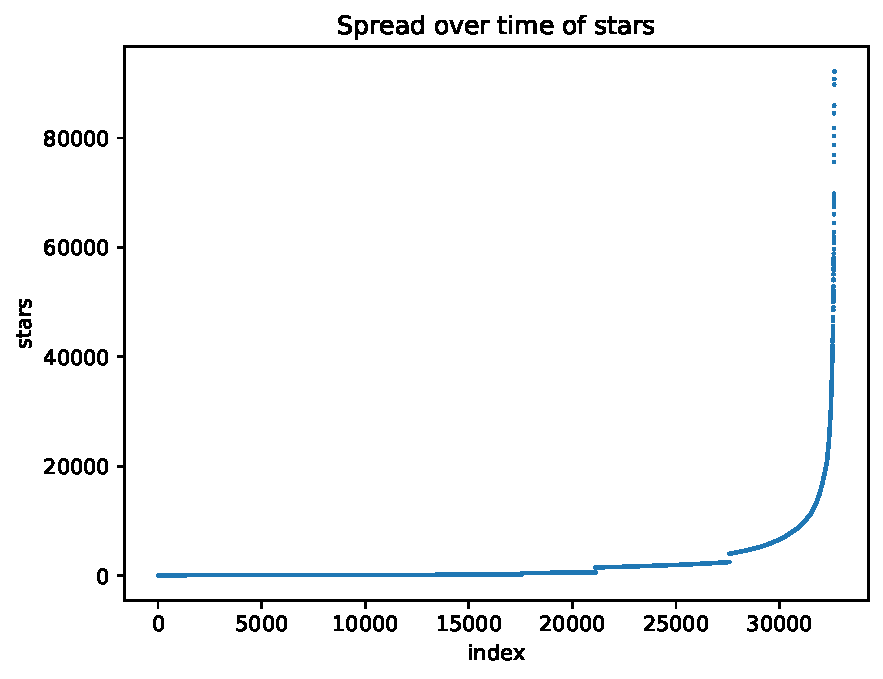
\includepdf[pages=-,pagecommand={},width=\textwidth]{../src/spread over time.pdf}

- what is the spread of ci/cd systems for public github repositories? this will take into account operating system, programming language, star count, subscriber count
- note: something along the lines of multiple configuration files
- what naming convention do they use for the files? (in order to understand common practices)





this will follow on from the previous graphs looking at spread of CI/CD configs found in the whole sample

then look at the difference that large repositories more than 100 commits with more than 2 contributors

then look at recent commits

perhaps a small look at naming conventions used???


\section{Config file results}

\vspace*{-0.05in}
\subsection{configuration errors when loading the config (just yaml parsing errors atm)}
\vspace*{-0.05in}

\begin {table}[!htbp]

\caption{Configuration types spread}
\label{table_config_types}
\begin{tabular}{lrl}
\hline
{} &  config & percentage \\ \hline

Travis          &   10607 &        74\% \\ \hline
Github          &    2301 &        16\% \\ \hline
CircleCi        &    1109 &         8\% \\ \hline
Jenkins pipeline &     161 &         1\% \\ \hline
Drone           &      84 &         1\% \\ \hline
Buildkite       &      32 &         0\% \\ \hline
Teamcity        &       4 &         0\% \\ \hline
Semaphore       &       2 &         0\% \\ \hline
Azure pipeline           &       1 &         0\% \\ \hline

\end{tabular}
\end{table}


\begin {table}[!htbp]

\caption{cats}
\begin{tabular}{|l|l|l|l|}
\hline
\textbf{yaml\_encoding\_error} &  composer error &  parse error &  scanner error \\ \hline
\textbf{config  } &                 &              &                \\ \hline

\textbf{circleci} &               0 &            0 &              1 \\ \hline
\textbf{drone   } &              30 &            0 &              0 \\ \hline
\textbf{github  } &               0 &            0 &              3 \\ \hline
\textbf{travis  } &               6 &           10 &             21 \\ \hline

\end{tabular}
\end{table}



\vspace*{-0.05in}
\subsection{How are comments used in configuration?}
\vspace*{-0.05in}

\vspace*{-0.05in}
\subsection{How are stages used in configuration?}
\vspace*{-0.05in}

and looking into branches

\vspace*{-0.05in}
\subsection{How are script tags used?}
\vspace*{-0.05in}

- how scripts with the configuration files? (need to elloborate more on this one)










By almost any measure, the Hubble Space Telescope scheduling problem
% is a complex task \cite{mj-early,sam}.
Between ten thousand and thirty thousand 
astronomical observations per year must be scheduled,
subject to a great
variety of constraints including
power restrictions, observation priorities,  
time-dependent orbital characteristics, 
movement of astronomical bodies, stray
light sources, etc. Because the telescope is an extremely
valuable resource with a limited lifetime, efficient scheduling
is a critical concern. An initial scheduling system, developed
using traditional programming methods,
highlighted the difficulty of the problem;
it was estimated that it would take over three
weeks for the system to schedule one
week of observations. As described in section \ref{results},
this problem was remedied by 
the development
of a successful constraint-based system to augment the initial system.
At the heart of the constraint-based system
is a neural network developed by Adorf and Johnston, 
the Guarded Discrete Stochastic (GDS) network,
% which searches for a schedule \cite{adorf,johnston}.

From a computational point of view the network is interesting because
Adorf and Johnston found that it performs well on a variety of tasks,
in addition to the space telescope scheduling problem. For example,
the network performs significantly better on the $n$-queens problem
than methods that were previously developed.  The $n$-queens problem
requires placing $n$ queens on an $n \times n$ chessboard so that no
two queens share a row, column or diagonal.  The network has been used
to solve problems of up to 1024 queens, whereas most heuristic
backtracking methods encounter difficulties with problems one-tenth
% that size \cite{stones}.

% The GDS network is a modified Hopfield network \cite{hopfield}. 
In a standard Hopfield network, all connections between neurons are
symmetric. In the GDS network, the main network is coupled
asymmetrically to an auxiliary network of {\em guard neurons} which
restricts the configurations that the network can assume.  This
modification enables the network to rapidly find a solution for many
problems, even when the network is simulated on a serial machine.  
Unfortunately, convergence to a stable configuration is no
longer guaranteed.  Thus the network can fall into a local minimum
involving a group of unstable states among which it will oscillate.
In practice, however, if the network fails to converge after some
number of neuron state transitions, it can simply be stopped and
started over.

To illustrate the network architecture and updating scheme, let us
consider how the network is used to solve binary constraint
satisfaction problems.  A problem consists of $n$ variables,
$X_{1}\ldots X_{n}$, with domains $D_{1}\ldots D_{n}$, and a set of
binary constraints. Each constraint $C_{\alpha}(X_{j},X_{k})$ is a
subset of $D_{j} \times D_{k}$ specifying incompatible values for a
pair of variables. The goal is to find an assignment for each of the
variables which satisfies the constraints. (In this paper we only
consider the task of finding a single solution, rather than that of
finding all solutions.)  To solve a CSP using the network, each
variable is represented by a separate set of neurons, one neuron for
each of the variable's possible values.  Each neuron is either ``on''
or ``off'', and in a solution state, every variable will have exactly
one of its corresponding neurons ``on'', representing the value of
that variable.  Constraints are represented by inhibitory (i.e.,
negatively weighted) connections between the neurons.  To insure that
every variable is assigned a value, there is a guard neuron for each
set of neurons representing a variable; if no neuron in the set is on,
the guard neuron will provide an excitatory input that is large enough
to turn one on.  (Because of the way the connection weights are set up, it
is unlikely that the guard neuron will turn on more than one neuron.)
The network is updated on each cycle by randomly picking a set of
neurons that represents a variable, and flipping the state of the
neuron in that set whose input is {\em most inconsistent} with its
current output (if any).  When all neurons' states are consistent with
their input, a solution is achieved.

  To solve the $n$-queens problem, for example, each of the $n \times n$ board
positions is represented by a neuron whose output is either one or
zero depending on whether a queen is currently placed in that position
or not.  (Note that this is a local representation rather than a
distributed representation of the board.)  If two board positions are
inconsistent, then an inhibiting connection exists between the
corresponding two neurons.  For example, all the neurons in a column
will inhibit each other, representing the constraint that two queens
cannot be in the same column.  For each row, there is a guard neuron
connected to each of the neurons in that row which gives the neurons
in the row a large excitatory input, enough so that at least one
neuron in the row will turn on.  The guard neurons thus enforce the
constraint that one queen in each row must be on.  As described above,
the network is updated on each cycle by randomly picking a row and
flipping the state of the neuron in that row whose input is most
inconsistent with its current output. A solution is realized when the
output of every neuron is consistent with its input.

\section{Why does the GDS Network Perform So Well?}
\label{mv-heuristic}

Our analysis of the GDS network was motivated by the following question:
``Why does the network perform so much better than traditional backtracking
methods on certain tasks''? In particular, we were intrigued by the results
on the $n$-queens problem, since this problem has received considerable
attention from previous researchers.  For $n$-queens, Adorf and Johnston
found empirically that the network requires a linear number of transitions to
converge. Since each transition requires linear time, the expected
(empirical) time for the network to find a solution is $O(n^2)$. To check
this behavior, Johnston and Adorf ran experiments with $n$ as high as 1024,
at which point memory limitations became a problem.\footnote{The network,
which is programmed in Lisp, requires approximately 11 minutes to solve the
1024 queens problem on a TI Explorer II. For larger problems, memory becomes
a limiting factor because the network requires approximately $O(n^{2})$
space.  (Although the number of connections is actually $O(n^{3})$, some
connections are computed dynamically rather than stored).}


\vspace*{-0.05in}
\subsection{Nonsystematic Search Hypothesis}
\vspace*{-0.05in}

Initially, we hypothesized that the network's advantage came from the
nonsystematic nature of its search, as compared to the systematic
organization inherent in depth-first backtracking. There are two
potential problems associated with systematic depth-first search.
First, the search space may be organized in such a way that poorer
choices are explored first at each branch point.  For instance, in the
$n$-queens problem, depth-first search tends to find a solution more
quickly when the first queen is placed in the center of the first row
rather than in the corner; apparently this occurs because
there are more solutions with the
% queen in the center than with the queen in the corner \cite{stones}.
Nevertheless,
most naive algorithms tend to start in the corner simply because
humans find it more natural to program that way.  However, this fact
by itself does not explain why nonsystematic search would work so well
for $n$-queens.  A backtracking program that randomly orders rows (and
columns within rows) performs much better than the naive method, but
still performs poorly relative to the GDS network.

\begin{figure}
\begin{center}
\setlength{\unitlength}{0.010in}
\begin{picture}(575,170)(15,465)

\put(255,480){\circle{10}}
\put(105,510){\circle{10}}
\put(205,510){\circle{10}}
\put( 95,510){\circle{10}}
\put(193,509){\circle{10}}
\put(115,510){\circle{10}}
\put(215,510){\circle{10}}
\put(510,510){\circle{10}}
\put(429,510){\circle{10}}
\put(469,510){\circle{10}}
\put(390,510){\circle{10}}
\put(550,510){\circle{10}}
\put(350,510){\circle{10}}
\put(255,550){\line( 1,-1){ 40}}
\put(255,550){\line( 1,-2){ 20}}
\put(255,550){\line( 0,-1){ 40}}
\put(225,550){\line( 1,-2){ 20}}
\put(225,550){\line( 1,-4){ 10}}
\put(225,550){\line( 0,-1){ 40}}
\put(205,550){\line( 1,-4){ 10}}
\put(205,550){\line( 0,-1){ 40}}
\put(205,550){\line(-1,-4){ 10}}
\put(105,550){\line( 1,-4){ 10}}
\put(105,550){\line( 0,-1){ 40}}
\put(105,550){\line(-1,-4){ 10}}
\put( 85,550){\line( 0,-1){ 40}}
\put( 85,550){\line(-1,-4){ 10}}
\put( 85,550){\line(-1,-2){ 20}}
\put( 55,550){\line( 0,-1){ 40}}
\put( 55,550){\line(-1,-2){ 20}}
\put( 55,550){\line(-1,-1){ 40}}
\put(215,590){\line( 1,-1){ 40}}
\put(215,590){\line( 1,-4){ 10}}
\put(175,590){\line( 3,-4){ 30}}
\put(175,590){\line( 0,-1){ 40}}
\put(135,590){\line( 0,-1){ 40}}
\put(135,590){\line(-3,-4){ 30}}
\put( 95,590){\line(-1,-4){ 10}}
\put( 95,590){\line(-1,-1){ 40}}
\put(155,630){\line( 1,-2){ 20}}
\put(155,630){\line( 3,-2){ 60}}
\put(155,630){\line(-1,-2){ 20}}
\put(155,630){\line(-3,-2){ 60}}
\put(135,550){\line(-1,-4){ 10}}
\put(135,550){\line( 1,-4){ 10}}
\put(175,550){\line( 1,-4){ 10}}
\put(175,550){\line(-1,-4){ 10}}
\put(175,550){\line( 0,-1){ 40}}
\put(135,550){\line( 0,-1){ 40}}
\put(430,550){\line( 0,-1){ 40}}
\put(470,550){\line( 0,-1){ 40}}
\put(470,550){\line(-1,-4){ 10}}
\put(470,550){\line( 1,-4){ 10}}
\put(430,550){\line( 1,-4){ 10}}
\put(430,550){\line(-1,-4){ 10}}
\put(450,630){\line(-3,-2){ 60}}
\put(450,630){\line(-1,-2){ 20}}
\put(450,630){\line( 3,-2){ 60}}
\put(450,630){\line( 1,-2){ 20}}
\put(390,590){\line(-1,-1){ 40}}
\put(390,590){\line(-1,-4){ 10}}
\put(430,590){\line(-3,-4){ 30}}
\put(430,590){\line( 0,-1){ 40}}
\put(470,590){\line( 0,-1){ 40}}
\put(470,590){\line( 3,-4){ 30}}
\put(510,590){\line( 1,-4){ 10}}
\put(510,590){\line( 1,-1){ 40}}
\put(350,550){\line(-1,-1){ 40}}
\put(350,550){\line(-1,-2){ 20}}
\put(350,550){\line( 0,-1){ 40}}
\put(380,550){\line(-1,-2){ 20}}
\put(380,550){\line(-1,-4){ 10}}
\put(380,550){\line( 0,-1){ 40}}
\put(400,550){\line(-1,-4){ 10}}
\put(400,550){\line( 0,-1){ 40}}
\put(400,550){\line( 1,-4){ 10}}
\put(500,550){\line(-1,-4){ 10}}
\put(500,550){\line( 0,-1){ 40}}
\put(500,550){\line( 1,-4){ 10}}
\put(520,550){\line( 0,-1){ 40}}
\put(520,550){\line( 1,-4){ 10}}
\put(520,550){\line( 1,-2){ 20}}
\put(550,550){\line( 0,-1){ 40}}
\put(550,550){\line( 1,-2){ 20}}
\put(550,550){\line( 1,-1){ 40}}
\end{picture}
\end{center} 
\caption{Solutions Clustered vs. Solutions Evenly Distributed}
\label{shotgun}
\end{figure}


The second potential problem with depth-first search is more significant
and more subtle. As illustrated by figure \ref{shotgun}, a depth-first
search can be a
disadvantage when solutions are not evenly distributed throughout the
search space.  In the tree at the left of the figure, the solutions 
are clustered together. In the tree on the right,
the solutions are more evenly distributed. Thus, the average distance
between solutions is greater in the left tree.  In a depth-first
search, the average time to find the first solution 
increases with the average distance between solutions. Consequently
depth-first search performs relatively poorly in a tree where
% the solutions are clustered, such as that on the left \cite{ginsberg,langley}.
In comparison,
a search strategy which examines the leaves of the tree in random
order is unaffected by solution clustering.

We investigated whether this phenomenon explained the relatively poor
performance 
of depth-first search on $n$-queens by experimenting with a randomized
% search algorithm, called a Las Vegas algorithm \cite{brassard}.  The
algorithm begins by selecting a path from the root to a leaf. To
select a path, the algorithm starts at the root node and chooses one
of its children with equal probability. This process continues
recursively until a leaf is encountered.  If the leaf is a solution
the algorithm terminates, if not, it starts over again at the root and
selects a path. The same path may be examined more than once, since
no memory is maintained between successive trials.

The Las Vegas algorithm does, in fact, perform better than simple
depth-first search on $n$-queens %\cite{brassard}.
However, the performance of the Las
Vegas algorithm is still not nearly as good as that of the GDS
network, and so we concluded that the systematicity hypothesis alone
cannot explain the network's behavior.

\subsection{Informedness Hypothesis}

Our second hypothesis was that the network's search process uses
information about the current assignment
that is not available to a constructive backtracking program.
's use of an iterative
improvement strategy guides the search in a way that is not possible
with a standard backtracking algorithm. 
We now believe this hypothesis
is correct, in that it explains why the network works so well.  In
particular, the key to the network's performance appears to be that
state transitions are made so as to reduce the number of outstanding
inconsistencies in the network; specifically, each state transition involves
flipping the neuron whose output is most
inconsistent with its current input. From a constraint satisfaction
perspective, it is as if the network reassigns a value for a variable
by choosing the value that violates the fewest constraints.
This idea is captured by the following heuristic:

{\small
\begin{quote}
{\bf Min-Conflicts heuristic:}\\
{\em Given:} A set of variables, a set of binary constraints, 
and an assignment specifying a value for each variable. 
Two variables {\em conflict} if their values violate a constraint.\\
{\em Procedure:} Select a variable that is in conflict,
and assign it a value that minimizes the number of conflicts.
(Break ties randomly.)
\end{quote}
}

We have found that the network's behavior can be approximated by a
symbolic system that uses the min-conflicts heuristic for
hill climbing.  The hill-climbing system starts with an initial
assignment generated in a preprocessing phase.  At each choice point,
the heuristic chooses a variable that is currently in conflict and
reassigns its value, until a solution is found. The system thus
searches the space of possible assignments, favoring assignments with
fewer total conflicts.  Of course, the hill-climbing system can become
``stuck'' in a local maximum, in the same way that the network may
become ``stuck'' in a local minimum.  In the next section we present
empirical evidence to support our claim that the min-conflicts
approach can account for the network's effectiveness.

   There are two aspects of the min-conflicts hill-climbing method
that distinguish it from standard CSP algorithms.
First, instead of incrementally constructing a consistent partial
assignment, the min-conflicts method {\em repairs} a complete but
inconsistent assignment by reducing inconsistencies.  Thus, it uses
information about the current assignment to guide its search that is
not available to a standard backtracking algorithm. Second,
the use of a hill-climbing strategy rather than a backtracking strategy
produces a different style of search.

\begin{figure}
{\small
{\bf
\begin{verbatim}
     Procedure INFORMED-BACKTRACK (VARS-LEFT VARS-DONE)
      If all variables are consistent, then solution found, STOP.
      Let VAR = a variable in VARS-LEFT that is in conflict.
      Remove VAR from VARS-LEFT.
      Push VAR onto VARS-DONE.
      Let VALUES = list of possible values for VAR in ascending order according 
                   to number of conflicts with variables in VARS-LEFT.
      For each VALUE in VALUES, until solution found:
        If VALUE does not conflict with any variable that is in VARS-DONE, 
        then Assign VALUE to VAR.
             Call INFORMED-BACKTRACK(VARS-LEFT VARS-DONE)
        end if
      end for
     end procedure
    
    Begin program
     Let VARS-LEFT = list of all variables, each assigned an initial value.
     Let VARS-DONE = nil
     Call INFORMED-BACKTRACK(VARS-LEFT VARS-DONE)
    End program
    \end{verbatim}
}
}
\caption{Informed Backtracking Using the Min-Conflicts Heuristic}
\label{iback}
\end{figure}



\subsubsection{Repair-Based Search Strategies}

(This is a example of a third level section.)
Extracting the method from the network enables us
to tease apart and experiment with its different components.
In particular, the idea of repairing an inconsistent assignment
can be used with a variety of different search strategies
in addition to hill climbing.
For example, we can backtrack through the space of possible repairs,
rather than using a hill-climbing strategy, as follows.
Given an initial assignment generated in a preprocessing phase, 
we can employ the min-conflicts
heuristic to order the choice of variables and values to consider,
as described in figure \ref{iback}.
Initially, the variables are all on a list
of {\sc vars-left}, and as they are repaired, they are pushed onto a 
list of {\sc vars-done}. 
The algorithm attempts
to find a sequence of repairs, such that no variable is repaired more than
once. If there is no way to repair a variable in {\sc vars-left} without
violating a previously repaired variable (a variable in {\sc vars-done}),
the algorithm backtracks.

Notice that this algorithm is simply a standard
backtracking algorithm augmented with the min-conflicts heuristic to
order its choice of which variable and value to attend to.  This
illustrates an important point. The backtracking repair algorithm
incrementally extends a consistent partial assignment (i.e., {\sc
vars-done}), as does a constructive backtracking program, but in addition,
uses information from the initial assignment (i.e., {\sc vars-left})
to bias its search. Thus, it is a type of {\em informed backtracking}.
We still characterize it as repair-based method since its search
is guided by a complete, inconsistent assignment.


\section{Experimental Results}

\label{results}

 [section ommitted]

\section{A Theoretical Model}
\label{analysis}

 [section ommitted]

\section{Discussion}

 [section ommitted]

\section{Acknowledgement}
The authors wish to thank Hans-Martin Adorf, Don Rosenthal, 
Richard Franier, Peter Cheeseman and Monte Zweben for their assistance
and advice.  We also thank Ron Musick and our anonymous reviewers for
their comments.  The Space Telescope Science Institute is operated by
the Association of Universities for Research in Astronomy for NASA.

\appendix
\section*{Appendix A. Probability Distributions for N-Queens}


[section ommitted]



\vskip 0.2in
\bibliography{sample}
\bibliographystyle{kentHarvard}

\end{document}
